\section{Blockwise Adaptive Huffmancoding}

Net zoals bij het \emph{Sliding window}-algoritme werd bij dit algoritme ook de \emph{blokgrootte} empirisch bepaald. Dezelfde bestanden als bij de \emph{Sliding window}-experimenten werden gebruikt, maar de grootteorden van de blokgroottes liggen vele malen hoger. Uit de tests volgt dat de optimale blokgrootte vastgelegd kan worden rond \SI{262144}{\byte}, het minimum van de grafiek in figuur \ref{fig:blocksize}.

\begin{figure}[h]
	\centering
	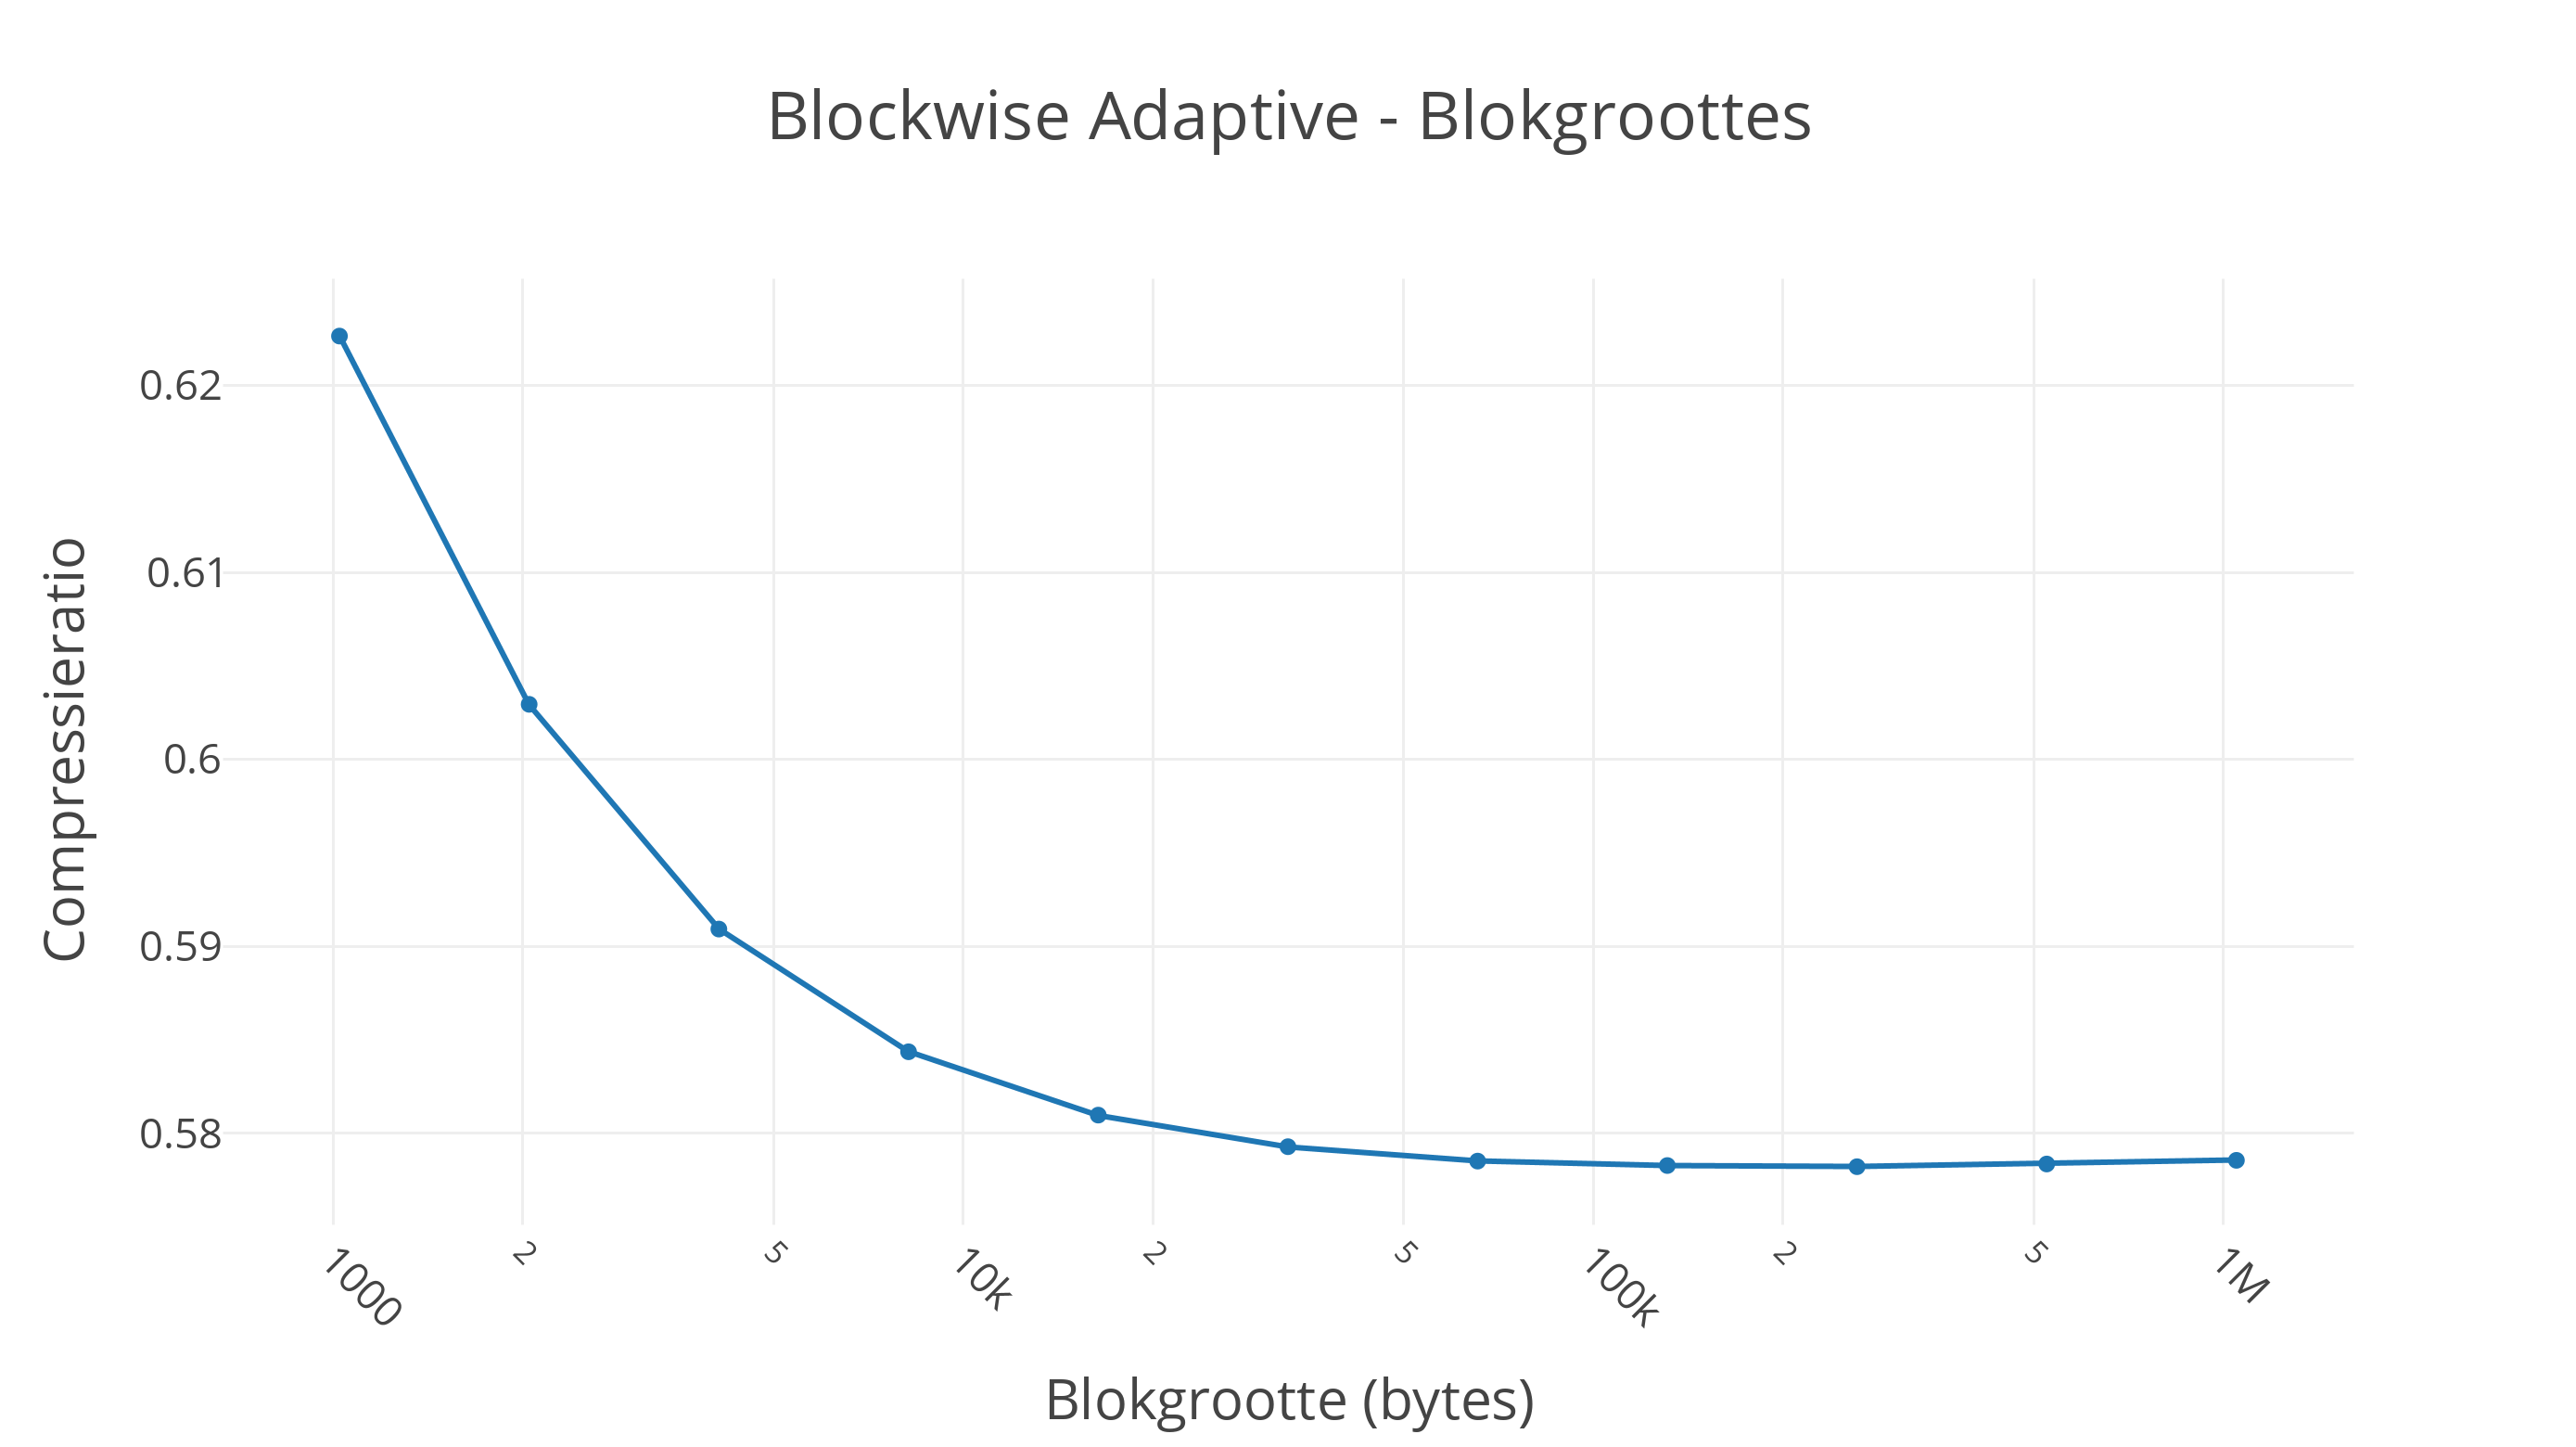
\includegraphics[width=0.9\linewidth]{resources/blockwise-size.png}
	\label{fig:blocksize}
	\caption{Vergelijking tussen verschillende blokgroottes}
\end{figure}